\documentclass[a4paper,11pt]{article}

\usepackage[utf8]{inputenc} %encodage
\usepackage[T1]{fontenc} %encodage alphabet accentué
\usepackage{lmodern} %police moderne
\usepackage{vmargin} %marge avancé
\usepackage[french]{babel} %standardisation du français
\usepackage{graphicx}
\usepackage{pdflscape}

%Mise en page
\oddsidemargin = 2cm
\evensidemargin = 2cm
\textwidth = 17cm
\topmargin = 7mm
\setlength{\textheight}{27cm}

\titlepage{
	\title{Rapport d'implémentations de Bartender}
	\date{\today}
	\author{Groupe Q}
}

\begin{document}

{\let\newpage\relax\maketitle}

Ce document reprend les modifications que nous avons du apporter à nos modèles de développement rendu au travail deux afin d'implémenter une application fonctionnelle.

\section{Diagramme UML}

\begin{itemize}
	\item Ajout de la méthode \textit{getBoissonFromNo()} dans la classe \texttt{Boisson}.
	\item Ajout de la méthode \textit{getProduitFromNo()} dans la classe \texttt{Inventaire}.
\end{itemize}

\section{Diagramme ORM}

\begin{itemize}
	\item Déplacement de l'attribut \textit{DéjàPayé} de la classe \texttt{Facture} vers \texttt{Détail}.
	\item Changement du type de l'attribut \textit{Photo} dans la classe \texttt{Boisson} de Blob vers String.
	\item Ajout de l'attribut \textit{DescriptionEN} dans la classe \texttt{Boisson}.
\end{itemize}

\begin{landscape}
\scalebox{0.4}{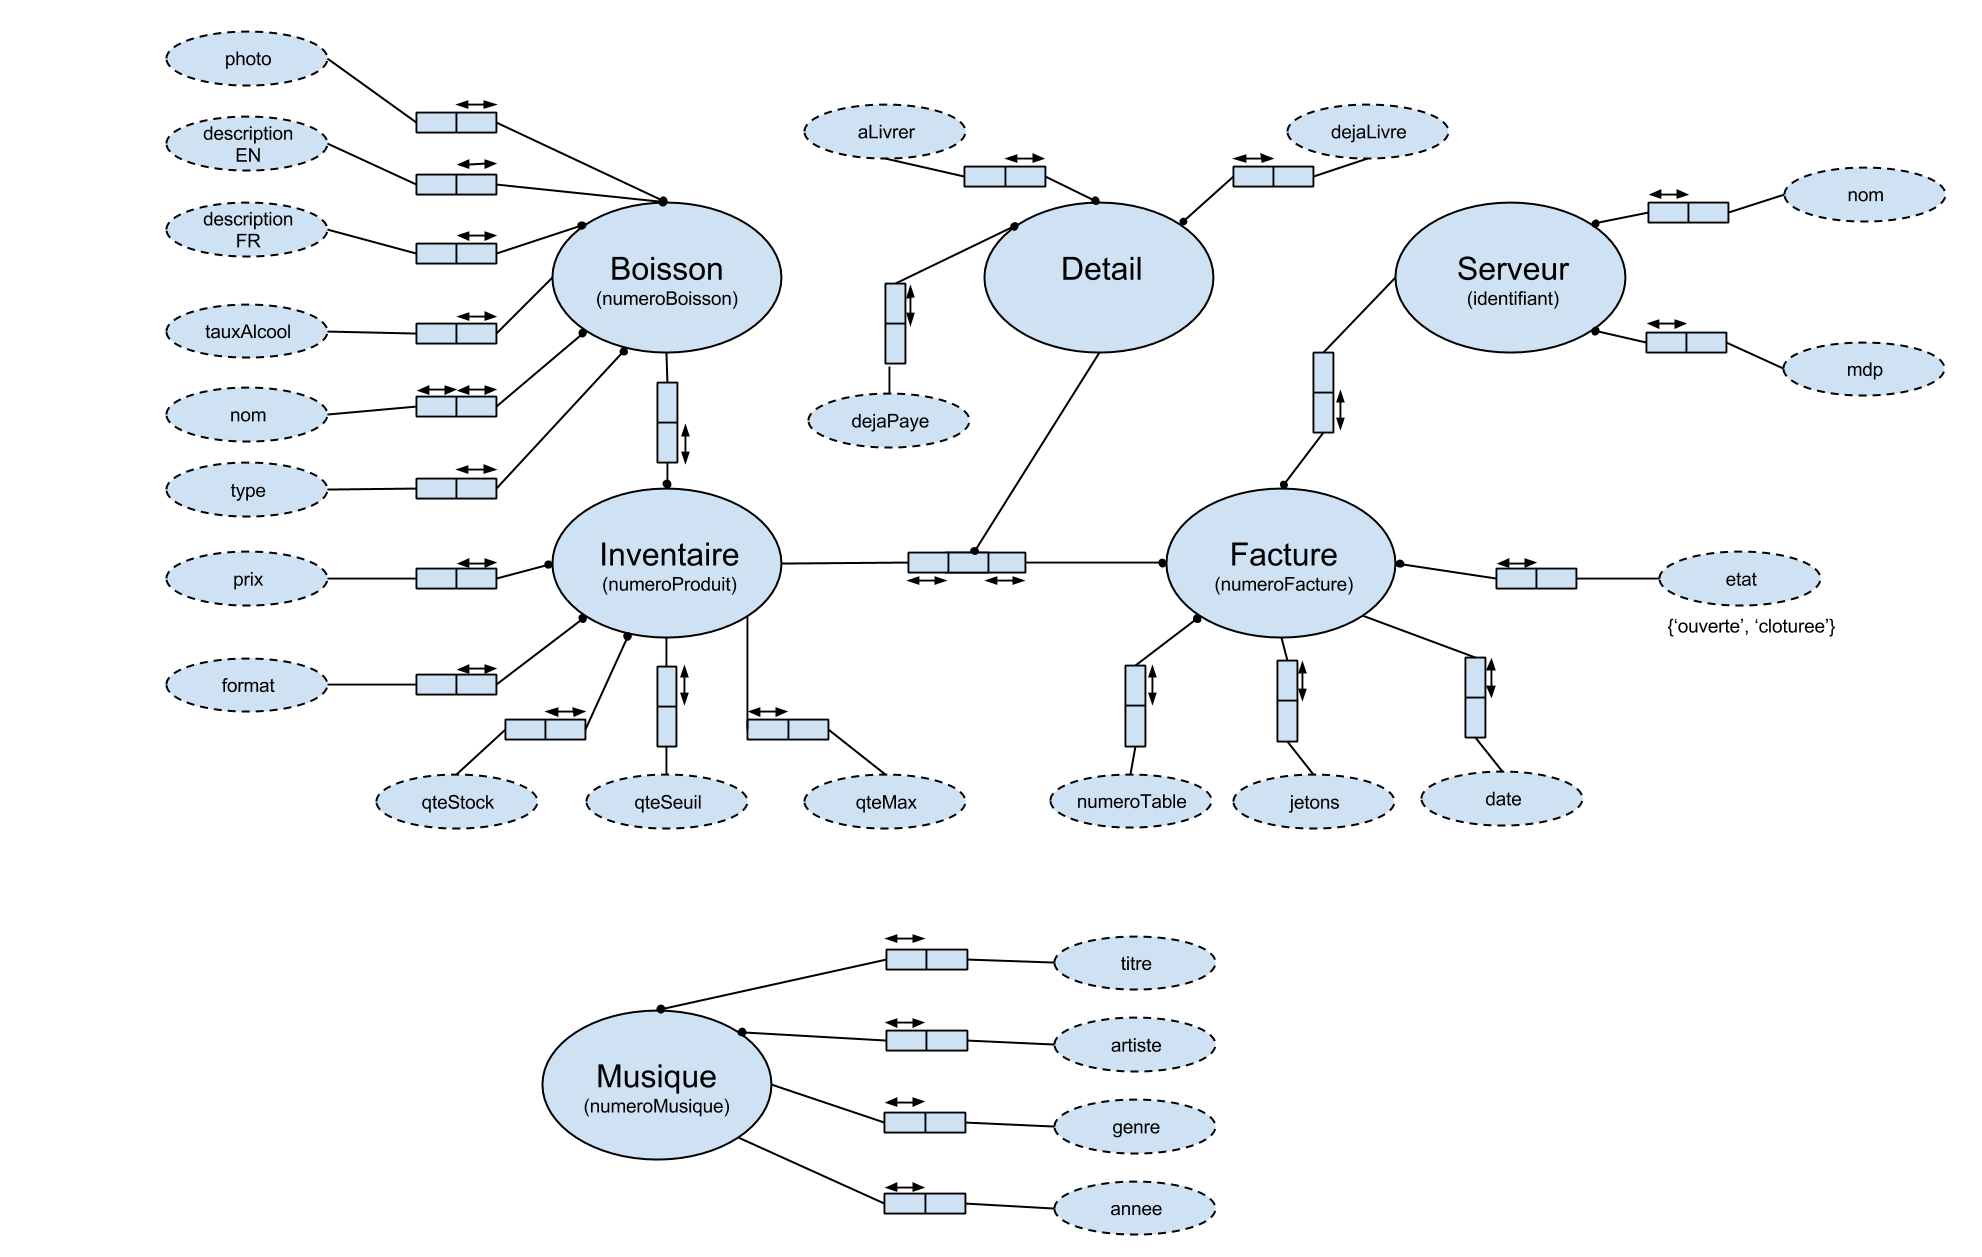
\includegraphics{ORM.png}}
\hspace*{1.25cm}
\scalebox{0.7}{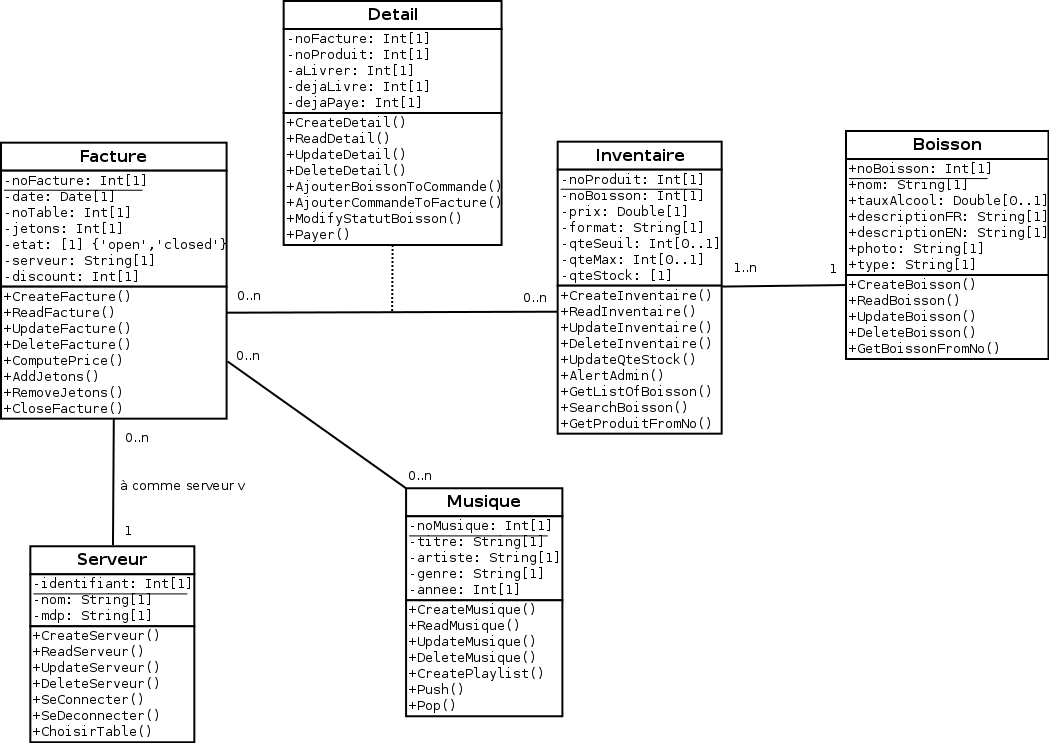
\includegraphics{UML.png}}
\end{landscape}

\end{document}